\section{Uncertainty and feasibility}\label{app:uncertainty}
\subsection{Conditional geometric bounds}
Let $\|v\|_s=\max_j|v_j|/s_j$, $d_t=\|x_t-x_t^0\|_s$ and $c_t=\|y_t-r_t\|_s$. If $\|x_t^0-r_t\|_s\le b_t$ and $\|n_t\|_s\le\eta_t$, the triangle and reverse triangle inequalities give
\begin{equation}
 \max(0,c_t-b_t-\eta_t)\le d_t\le c_t+b_t+\eta_t.\label{eq:bound}
\end{equation}
Scalar errors aligned in the same direction attain these extremes. For coordinate error boxes with half-widths $b_{t,j},\eta_{t,j}$, return within $\delta$ holds for every admissible pair exactly when
\begin{equation}
 \max_j\frac{|y_{t,j}-r_{t,j}|+b_{t,j}+\eta_{t,j}}{s_j}\le\delta.\label{eq:box}
\end{equation}
Each coordinate can attain the summed magnitude, proving necessity as well as sufficiency. If any $b_{t,j}+\eta_{t,j}>\delta s_j$, the condition is infeasible. E1 instead tests $c_t+b\le\delta$ with a maximum observed normal discrepancy $b$. That maximum combines model error and noise; Gaussian noise is unbounded. The tested rule is therefore an empirical heuristic, not a verified certificate. Dwell cannot repair $b>\delta$.

\subsection{Covariance-aware window evidence}
For dimensionless residuals write $e_{t,j}=v_{t,j}+\beta_{t,j}+\epsilon_{t,j}$, with $|\beta_{t,j}|\le B_j$ and $|v_{t,j}-v_{t-1,j}|\le L_j$. Assume stationary zero-mean Gaussian AR(1) noise with marginal standard deviation $\sigma_j$ and correlation $0\le\rho_j<1$. Its window-mean variance is
\begin{equation}
 V_{m,j}=\frac{\sigma_j^2}{m^2}\left[m+2\sum_{k=1}^{m-1}(m-k)\rho_j^k\right].\label{eq:covariance}
\end{equation}
For $K$ registered windows and $d$ channels, allocate $\alpha_t=6\alpha/(\pi^2t^2)$ on a clock that never restarts at alarms, and define
\begin{align}
 U_{t,j}(m)={}&|\bar e_{t,j}(m)|+B_j+\frac{L_j(m-1)}2\nonumber\\
 &+\sqrt{2V_{m,j}\log(2dK/\alpha_t)}.\label{eq:windowbound}
\end{align}
With probability at least $1-\alpha$, $|v_{t,j}|\le U_{t,j}(m)$ for every channel, complete registered window and prospective time within a trace. Thus coordinatewise return is certified on that event if
\begin{equation}
 \min_{m\in\mathcal M}U_{t,j}(m)\le\delta_j\quad\text{for every }j.\label{eq:certificate}
\end{equation}
To verify the claim, the two-sided Gaussian tail is at most $\alpha_t/(dK)$. A union bound over channels, windows and times uses $\sum_t\alpha_t=\alpha$. Window overlap and cross-channel dependence do not invalidate that bound. Finally, $|v_{t,j}-\bar v_{t,j}(m)|\le L_j(m-1)/2$ and $|\bar\beta|\le B_j$ yield Equation~\ref{eq:windowbound}. Different channels may select different windows because all bounds hold simultaneously.

This is elementary error spending under supplied assumptions, not new confidence-sequence theory. Invalid observations invalidate affected windows without resetting time. Failure to certify leaves return uncertain and does not generate an attack alarm. Unknown covariance, heavy tails or nonstationarity fall outside the guarantee.

\subsection{Residual experiment and complete results}
E4 fixes $d=4$, windows $\{1,41,201\}$, $\alpha=0.05$, tolerance 0.1 and bias bound 0.01. The four $(\sigma,\rho)$ settings are $(0.03,0)$, $(0.06,0)$, $(0.03,0.8)$ and $(0.06,0.95)$, with channel multipliers $(1,0.8,1.1,0.9)$. Bias is $0.01\cos(0.003t+\phi_j)$ for phases $(0,0.4,0.8,1.2)$. Deviation is zero, $0.02\sin(0.004t+\phi_j)$, or $0.02\sin(0.04t+\phi_j)$; its supplied increment bound is $2a|\sin(\omega/2)|$.

Each trace has 1,200 points and stationary initial noise. Seeds 17, 42 and 2026 supply paired innovations across settings, producing 36 constructed traces. Common support is points 201--1,200. Three fixed-window controls and their simultaneous envelope receive identical residuals/bounds; two deliberately misspecified controls set $\rho=0$ for windows 41 and 201. All 216 outcomes remain recorded. The envelope must certify at least 95\% of common points on every trace. The per-trace probability statement is not simultaneous 95\% coverage across the experiment matrix.

\begin{table*}[t]\centering
\caption{E4 simultaneous-envelope certificates on normal synthetic residuals. Ranges span three seeds with 1,000 common points each. Every trace must reach 95\%; the overall criterion fails.}\label{tab:window}
\begin{tabular}{llrr}\toprule
Noise setting & Deviation profile & Certificates (\%) & Passes \\\midrule
Independent, low & Settled & 100.0--100.0 & 3/3 \\
Independent, low & Slow variation & 100.0--100.0 & 3/3 \\
Independent, low & Faster variation & 100.0--100.0 & 3/3 \\
Independent, high & Settled & 100.0--100.0 & 3/3 \\
Independent, high & Slow variation & 100.0--100.0 & 3/3 \\
Independent, high & Faster variation & 17.2--25.6 & 0/3 \\
Correlated, low & Settled & 100.0--100.0 & 3/3 \\
Correlated, low & Slow variation & 85.8--100.0 & 2/3 \\
Correlated, low & Faster variation & 0.0--0.0 & 0/3 \\
Correlated, high & Settled & 0.0--0.0 & 0/3 \\
Correlated, high & Slow variation & 0.0--0.0 & 0/3 \\
Correlated, high & Faster variation & 0.0--0.0 & 0/3 \\
\bottomrule\end{tabular}

\end{table*}
\begin{figure*}[t]\centering
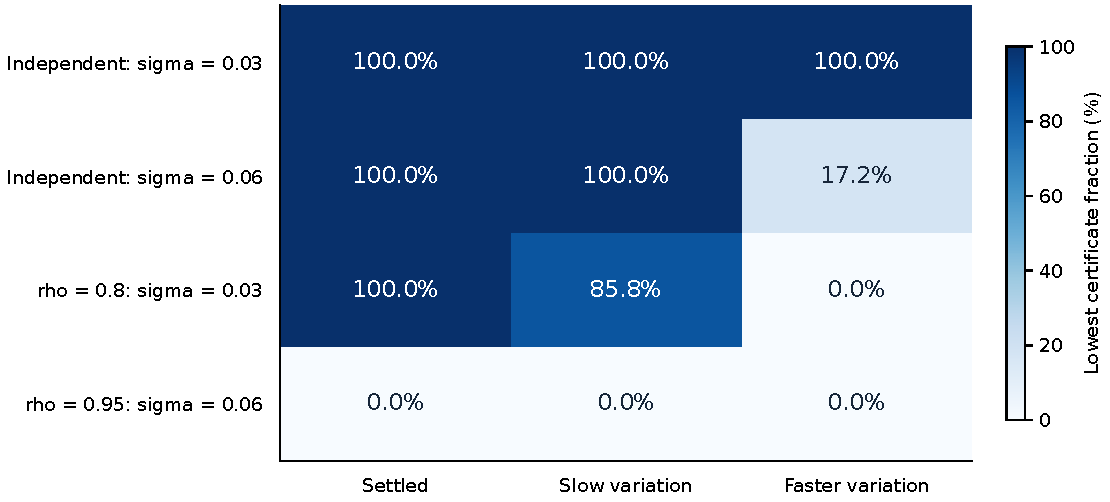
\includegraphics[width=0.62\textwidth]{figures/window_feasibility.pdf}
\caption{Lowest E4 certificate fraction across seeds in each residual condition. All true deviations lie within tolerance. Low certificate coverage means uncertain return under the supplied bounds, not detected attacks.}\label{fig:window}
\end{figure*}

The envelope passes 20/36 traces. Instantaneous evidence certifies none. Under independent low noise with faster variation, window 41 certifies every point while 201 certifies none: the longer drift allowance outweighs averaging. Under correlated low noise with slow variation, fractions are 100\%, 85.8\% and 100\%; their 95.27\% average does not satisfy the all-traces rule. At $(0.06,0.95)$ no valid control certifies even settled motion. The misspecified 201-point control would certify 91.53\% on average there, without a valid covariance guarantee.

This generator constructs residuals directly and supplies the bounds; it does not simulate robot dynamics or attacks. All deviations are within tolerance, so the absence of observed bound violations cannot establish rare unsafe-clearing risk. Operational estimation of the assumptions and behavior near the tolerance boundary remain untested.
